\documentclass[t]{beamer}
\usetheme{Copenhagen}
\setbeamertemplate{headline}{} % remove toc from headers
\beamertemplatenavigationsymbolsempty

\usepackage{amsmath, array, tikz, bm, pgfplots, tcolorbox, graphicx, venndiagram, color, colortbl}
\pgfplotsset{compat = 1.16}
\usepgfplotslibrary{statistics}
\usetikzlibrary{trees}

\title{Qualitative Graphs}
\author{}
\date{}

\AtBeginSection[]
{
  \begin{frame}
    \frametitle{Objectives}
    \tableofcontents[currentsection]
  \end{frame}
}

\begin{document}

\begin{frame} 
\maketitle
\end{frame}

\begin{frame}{Why Bother with a Graph?}
With all of the tools and techniques available for working with data, why should we bother to obtain a visualizaiton of it?	\newline\\	\pause

Can provide you with all of the data regarding a car: make, model, color, mileage, maintenance and repair history, etc. but ultimately...	\pause
\begin{center}
\color{blue}\textbf{You would want to know at least know what it looks like.}
\end{center}
\vspace{10pt}	\pause
The same principal can be applied to datasets.
\end{frame}

\section{Create and interpret bar graphs}

\begin{frame}{Bar Graphs}
\begin{tcolorbox}[colframe=green!20!black, colback = green!30!white,title=\textbf{Bar Graph}]
A \textbf{bar graph} is a visual display of data in which bars are plotted, where one dimension represents each category and the other dimension represents the frequency (or relative frequency) of each category.
\end{tcolorbox}
\vspace{6pt}	\pause
\begin{center}
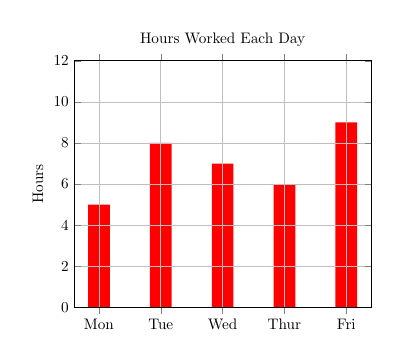
\begin{tikzpicture}[scale=0.55]
\begin{axis}[
ybar, axis on top, title={Hours Worked Each Day}, bar width = 0.5cm, grid,
ymin = 0, ymax = 12, ylabel = {Hours},
symbolic x coords = {Mon, Tue, Wed, Thur, Fri}, xtick=data
]
\addplot [draw=none, fill=red] coordinates{
	(Mon,5) (Tue,8) (Wed,7) (Thur,6) (Fri,9)
};
\end{axis}
\end{tikzpicture}
\end{center}
\end{frame}

\begin{frame}{Bar Graphs}
Bar graphs can be clustered:	\newline\\
\begin{center}
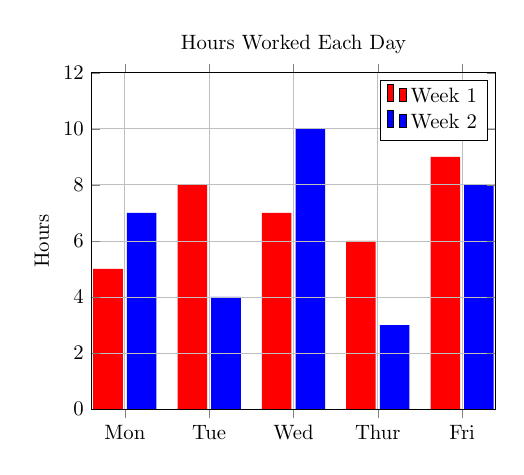
\begin{tikzpicture}[scale=0.75]
\begin{axis}[
ybar, axis on top, title={Hours Worked Each Day}, bar width = 0.5cm, grid,
ymin = 0, ymax = 12, ylabel = {Hours}, legend entries = {Week 1, Week 2},
symbolic x coords = {Mon, Tue, Wed, Thur, Fri}, xtick=data
]
\addplot [draw=none, fill=red] coordinates{
	(Mon,5) (Tue,8) (Wed,7) (Thur,6) (Fri,9)
};
\addplot [draw=none, fill=blue] coordinates{
	(Mon,7) (Tue,4) (Wed,10) (Thur,3) (Fri,8)
};
\end{axis}
\end{tikzpicture}
\end{center}
\end{frame}

\begin{frame}{Bar Graphs}
Bar graphs can be stacked:	\newline\\
\begin{center}
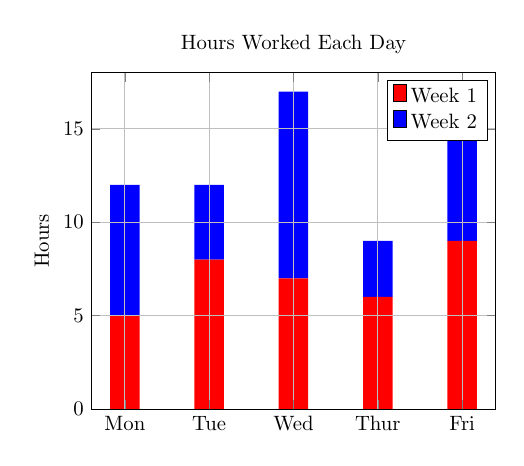
\begin{tikzpicture}[scale=0.75]
\begin{axis}[
ybar stacked, axis on top, title={Hours Worked Each Day}, bar width = 0.5cm, grid,
ymin = 0, ymax = 18, ylabel = {Hours}, legend entries = {Week 1, Week 2},
symbolic x coords = {Mon, Tue, Wed, Thur, Fri}, xtick=data
]
\addplot [draw=none, fill=red] coordinates{
	(Mon,5) (Tue,8) (Wed,7) (Thur,6) (Fri,9)
};
\addplot [draw=none, fill=blue] coordinates{
	(Mon,7) (Tue,4) (Wed,10) (Thur,3) (Fri,8)
};
\end{axis}
\end{tikzpicture}
\end{center}
\end{frame}

\begin{frame}{Bar Graphs}
Bar graphs can be horizontal:	\newline\\
\begin{center}
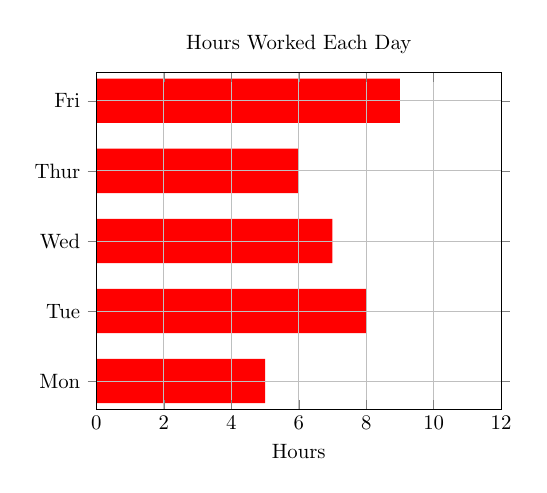
\begin{tikzpicture}[scale=0.75]
\begin{axis}[
xbar, axis on top, title={Hours Worked Each Day}, bar width = 0.75cm, grid,
xmin = 0, xmax = 12, xlabel = {Hours},
symbolic y coords = {Mon, Tue, Wed, Thur, Fri}, ytick=data
]
\addplot [draw=none, fill=red] coordinates{
	(5,Mon) (8,Tue) (7,Wed) (6,Thur) (9,Fri)
};
\end{axis}
\end{tikzpicture}
\end{center}
\end{frame}

\begin{frame}{Bar Graphs}
Bar graphs can show relative frequency (percent of total):	\newline\\
\begin{center}
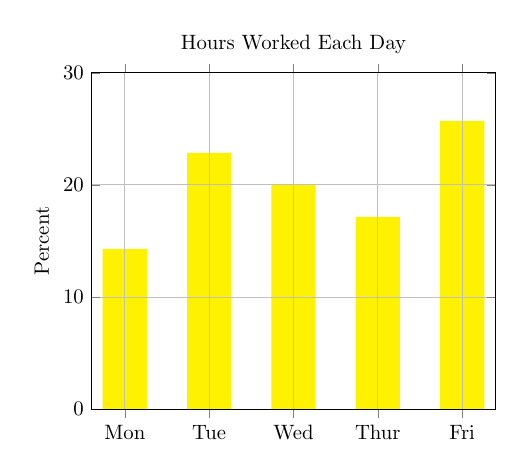
\begin{tikzpicture}[scale=0.75]
\begin{axis}[
ybar, axis on top, title={Hours Worked Each Day}, bar width = 0.75cm, grid,
ymin = 0, ymax = 30, ylabel = {Percent},
symbolic x coords = {Mon, Tue, Wed, Thur, Fri}, xtick=data
]
\addplot [draw=none, fill=yellow] coordinates{
	(Mon,14.29) (Tue,22.86) (Wed,20) (Thur,17.14) (Fri,25.71)
};
\end{axis}
\end{tikzpicture}
\end{center}
\end{frame}

% : Freq & Rel freq
% Pareto charts & ogives
% Create and interpret pie graphs

\end{document}